\documentclass[11pt,a4paper]{article}
\usepackage[T1]{fontenc}
\usepackage[left=2cm, right=2cm, top=2cm, bottom=2cm]{geometry}
\usepackage{graphicx}
\usepackage{mathtools}
\usepackage{amssymb}
\usepackage{amsthm}
\usepackage{thmtools}
\usepackage{xcolor}
\usepackage{nameref}
\usepackage{hyperref}
\usepackage{physics}
\usepackage{amsmath}
\usepackage{tikz}
\usepackage{mathdots}
\usepackage{yhmath}
\usepackage{cancel}
\usepackage{color}
\usepackage{siunitx}
\usepackage{array}
\usepackage{multirow}
\usepackage{amssymb}
\usepackage{gensymb}
\usepackage{tabularx}
\usepackage{extarrows}
\usepackage{booktabs}
\usetikzlibrary{fadings}
\usetikzlibrary{patterns}
\usetikzlibrary{shadows.blur}
\usetikzlibrary{shapes}

\usepackage{placeins}








\title{A Second Chance For Random Varaibles}
\author{Ali Fele Paranj}

\newtheoremstyle{Example}
{\topsep}   % Space above
{\topsep}   % Space below
{}  % Body font
{}          % Indent amount
{\bfseries} % Theorem head font (bold)
{.}         % Punctuation after theorem head
{ }         % Space after theorem head
{}          % Theorem head spec


\theoremstyle{Example}
\newtheorem{example}{Example}

\newcommand{\N}{\mathbb{N}}





\begin{document}
	\maketitle
	\begin{abstract}
		To me, the notion of random variables is something that I learn a new aspect of it as I encounter it in different situations. When I first learned the notion of random variable, it was already been abused by some physicists by the way that taught it to us (and it is most likely to be so to most of the people who learned it from non-mathematicians!). In this note I will explain some aspects of random variables through a running example. After this note you will have a clear understanding of the notion of random variables, martingales, filtration, and you will have an intuitive feeling about the statements like ``$\sigma\text{-algebra}$ can be thought of as information''.
	\end{abstract}
	
	
	
	\section*{Random Variables}
	We start with an example.
	
	\begin{example}
		Consider an experiment in which we toss a coin infinitely many times. The sample space $ \Omega $ for such experiment will be the $ \mathbb{F}_2^\N $, i.e. the set of all sequences composed of zeros and ones. We want to show that $ \Omega $ is ``similar'' to the interval $ (0,1] $ in interesting ways. Consider the partition $ \Omega = A_0 \cup A_1 $, where $ A_0 $ is the set of all outcomes that start with $ 0 $ and $ A_1 $ is the set of all outcomes that start with 1. Similarly we can have the partition $ \Omega = A_{00} \cup A_{01} \cup A_{10} \cup A_{11} $ where $ A_{01} $, for instance, is the set of all outcomes that start with $ 01 $. We can associate with, say, $ A_{01} $ a subset of $ (0,1] $ whose the dyadic expansion of all numbers in that interval starts with 01. For instance
		\[ A_{00} \mapsto (0,1/4], \qquad A_{01} \mapsto (1/4,1/2], \qquad A_{10} \mapsto (1/2,3/4], \qquad A_{11} \mapsto (3/4,1]. \]
	\end{example}
 	
 	The idea of probability theory is to remove all kind of randomness by considering as big state space as possible. For instance, assume you want to do an infinite coin toss experiment. From the probability theory point of view, the moment you start to do your experiment you will be some $ \omega \in \Omega $, for which every step of your coin tossing is known. In other words, any combination of outcomes that you might encounter in your experiment is already included in the sample space, thus any particular outcome you might get is a concrete element of the probability space. Now imagine the following story!
 	
 	\begin{example}
 		You are talking with one of your friends over phone and he says while he was speaking he just started random coin toss experiment (with a fail coin!). Then you feel peculiar as you look at the real line on the black board of your office and you know that he is now assigned to some $ \omega \in (0,1] $. But which one? You wish you know the exact point, then you could bet with your friend that you can predict the outcome of all of his coin tosses and you get a lot of money.
 	\end{example}
 	
 	So far, you should have believed that anybody anywhere in this universe, once they start a random coin toss experiment, then they are automatically assigned to one of the points $ \omega \in (0,1] $, as by definition $ \Omega $ is the set of all possible outcomes that when anybody anywhere in this universe, once they start a random coin toss experiment, their result is also included in $ \Omega $. But in probability theory, do not care about the outcome of the particular experiment of your friend, but we instead are interested in looking at all of the possible experiments all at once, and make important observations. This is very similar to the idea of ensembles in statistical physics.
 	
 	\begin{example}
 		You friend from previous example tells you that since he started doing the infinite coin tossing experiment, he wants to do something with it. He decides to choose some direction (the same direction for the entire infinite experiment) and then start moving back and forth on that line based on the result of each coin toss. 1 step forward for a heads and 1 step backward for a tails. Once you notice his strange decision you get nervous, because you don't know where he will end up to be in. So you decide to do something and calculate how far one can possibly go? For instance if your friends comes up with an outcome like $ (H,T,H,T,H,\cdots) $, then there is no danger since he wont be able to go very far. But what about all other cases?
 	\end{example}
 	
 	The answer of the question above might be complicated at first, but it is very straightforward given the identification we had before. E.g. you know that all the experiments that start with a patters line $ (H,\cdots) $ should belong to $ A_{1} \mapsto (1/2,1] $, and etc. So you start drawing the following \emph{dyadic functions}.
 	\begin{figure}[h!]
 		\centering
 		
 		
 		\tikzset{every picture/.style={line width=0.75pt}} %set default line width to 0.75pt        
 		
 		\begin{tikzpicture}[x=0.75pt,y=0.75pt,yscale=-1,xscale=1]
 			%uncomment if require: \path (0,300); %set diagram left start at 0, and has height of 300
 			
 			%Straight Lines [id:da4148364298012466] 
 			\draw [color={rgb, 255:red, 155; green, 155; blue, 155 }  ,draw opacity=1 ]   (130,100) -- (130,22) ;
 			\draw [shift={(130,20)}, rotate = 90] [color={rgb, 255:red, 155; green, 155; blue, 155 }  ,draw opacity=1 ][line width=0.75]    (10.93,-3.29) .. controls (6.95,-1.4) and (3.31,-0.3) .. (0,0) .. controls (3.31,0.3) and (6.95,1.4) .. (10.93,3.29)   ;
 			%Straight Lines [id:da5506235057459017] 
 			\draw [color={rgb, 255:red, 155; green, 155; blue, 155 }  ,draw opacity=1 ]   (120,60) -- (308,60) ;
 			\draw [shift={(310,60)}, rotate = 180] [color={rgb, 255:red, 155; green, 155; blue, 155 }  ,draw opacity=1 ][line width=0.75]    (10.93,-3.29) .. controls (6.95,-1.4) and (3.31,-0.3) .. (0,0) .. controls (3.31,0.3) and (6.95,1.4) .. (10.93,3.29)   ;
 			%Straight Lines [id:da1158916305978619] 
 			\draw    (210,40) -- (290,40) ;
 			%Straight Lines [id:da258390182805619] 
 			\draw    (130,80) -- (210,80) ;
 			%Straight Lines [id:da011923656679230454] 
 			\draw    (210,40) -- (210,80) ;
 			%Straight Lines [id:da08747010776417685] 
 			\draw    (290,40) -- (290,60) ;
 			%Straight Lines [id:da607559943652312] 
 			\draw    (130,60) -- (130,80) ;
 			
 		\end{tikzpicture}
 	\end{figure}
 	\FloatBarrier
 	\noindent The function above (a random variable!) is very simple, yet tells us a very important fact. This function ``reports'' the result of the very first step for all the experiments. The experiments in $ (0,1/2] $ will go one step backwards as their first outcome is a tails, and the experiments in $ (1/2,1] $ will go one step forward, as their first outcome is a heads. Cool! Then you continued doing this for the second, and the third step.
 	\begin{figure}[h!]
	\centering
	
	
	
	\tikzset{every picture/.style={line width=0.75pt}} %set default line width to 0.75pt        
	
	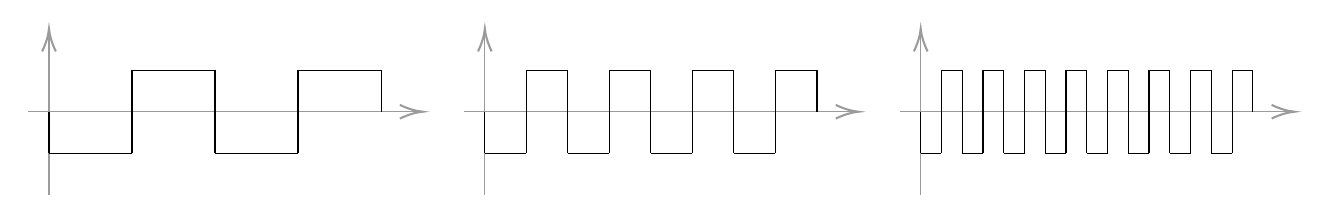
\begin{tikzpicture}[x=0.75pt,y=0.75pt,yscale=-1,xscale=1]
		%uncomment if require: \path (0,300); %set diagram left start at 0, and has height of 300
		
		%Straight Lines [id:da4148364298012466] 
		\draw [color={rgb, 255:red, 155; green, 155; blue, 155 }  ,draw opacity=1 ]   (20,160) -- (20,82) ;
		\draw [shift={(20,80)}, rotate = 90] [color={rgb, 255:red, 155; green, 155; blue, 155 }  ,draw opacity=1 ][line width=0.75]    (10.93,-3.29) .. controls (6.95,-1.4) and (3.31,-0.3) .. (0,0) .. controls (3.31,0.3) and (6.95,1.4) .. (10.93,3.29)   ;
		%Straight Lines [id:da5506235057459017] 
		\draw [color={rgb, 255:red, 155; green, 155; blue, 155 }  ,draw opacity=1 ]   (10,120) -- (198,120) ;
		\draw [shift={(200,120)}, rotate = 180] [color={rgb, 255:red, 155; green, 155; blue, 155 }  ,draw opacity=1 ][line width=0.75]    (10.93,-3.29) .. controls (6.95,-1.4) and (3.31,-0.3) .. (0,0) .. controls (3.31,0.3) and (6.95,1.4) .. (10.93,3.29)   ;
		%Straight Lines [id:da258390182805619] 
		\draw    (20,140) -- (60,140) ;
		%Straight Lines [id:da011923656679230454] 
		\draw    (60,100) -- (60,140) ;
		%Straight Lines [id:da08747010776417685] 
		\draw    (180,100) -- (180,120) ;
		%Straight Lines [id:da607559943652312] 
		\draw    (20,120) -- (20,140) ;
		%Straight Lines [id:da9293595573793709] 
		\draw    (60,100) -- (100,100) ;
		%Straight Lines [id:da30811722397795993] 
		\draw    (100,100) -- (100,140) ;
		%Straight Lines [id:da41636262903881516] 
		\draw    (100,140) -- (140,140) ;
		%Straight Lines [id:da11975040199452103] 
		\draw    (140,100) -- (140,140) ;
		%Straight Lines [id:da13481427607148566] 
		\draw    (140,100) -- (180,100) ;
		%Straight Lines [id:da026815163298576028] 
		\draw [color={rgb, 255:red, 155; green, 155; blue, 155 }  ,draw opacity=1 ]   (230,160) -- (230,82) ;
		\draw [shift={(230,80)}, rotate = 90] [color={rgb, 255:red, 155; green, 155; blue, 155 }  ,draw opacity=1 ][line width=0.75]    (10.93,-3.29) .. controls (6.95,-1.4) and (3.31,-0.3) .. (0,0) .. controls (3.31,0.3) and (6.95,1.4) .. (10.93,3.29)   ;
		%Straight Lines [id:da7149525315184728] 
		\draw [color={rgb, 255:red, 155; green, 155; blue, 155 }  ,draw opacity=1 ]   (220,120) -- (408,120) ;
		\draw [shift={(410,120)}, rotate = 180] [color={rgb, 255:red, 155; green, 155; blue, 155 }  ,draw opacity=1 ][line width=0.75]    (10.93,-3.29) .. controls (6.95,-1.4) and (3.31,-0.3) .. (0,0) .. controls (3.31,0.3) and (6.95,1.4) .. (10.93,3.29)   ;
		%Straight Lines [id:da38340551031671466] 
		\draw    (250,100) -- (250,140) ;
		%Straight Lines [id:da7742477612466505] 
		\draw    (390,100) -- (390,120) ;
		%Straight Lines [id:da17869669649468123] 
		\draw    (230,120) -- (230,140) ;
		%Straight Lines [id:da8457464963978909] 
		\draw    (230,140) -- (250,140) ;
		%Straight Lines [id:da6726082323376037] 
		\draw    (270,100) -- (270,140) ;
		%Straight Lines [id:da485239618048773] 
		\draw    (250,100) -- (270,100) ;
		%Straight Lines [id:da5974764605996938] 
		\draw    (290,100) -- (290,140) ;
		%Straight Lines [id:da39238301406358445] 
		\draw    (270,140) -- (290,140) ;
		%Straight Lines [id:da7254324281576592] 
		\draw    (310,100) -- (310,140) ;
		%Straight Lines [id:da15432691307682322] 
		\draw    (290,100) -- (310,100) ;
		%Straight Lines [id:da6608070418620688] 
		\draw    (330,100) -- (330,140) ;
		%Straight Lines [id:da4261703083983439] 
		\draw    (310,140) -- (330,140) ;
		%Straight Lines [id:da021919102262065282] 
		\draw    (350,100) -- (350,140) ;
		%Straight Lines [id:da6554788124199364] 
		\draw    (330,100) -- (350,100) ;
		%Straight Lines [id:da6124036117407075] 
		\draw    (370,100) -- (370,140) ;
		%Straight Lines [id:da37130833770131466] 
		\draw    (350,140) -- (370,140) ;
		%Straight Lines [id:da3332834004619616] 
		\draw    (370,100) -- (390,100) ;
		%Straight Lines [id:da39307763949721286] 
		\draw [color={rgb, 255:red, 155; green, 155; blue, 155 }  ,draw opacity=1 ]   (440,160) -- (440,82) ;
		\draw [shift={(440,80)}, rotate = 90] [color={rgb, 255:red, 155; green, 155; blue, 155 }  ,draw opacity=1 ][line width=0.75]    (10.93,-3.29) .. controls (6.95,-1.4) and (3.31,-0.3) .. (0,0) .. controls (3.31,0.3) and (6.95,1.4) .. (10.93,3.29)   ;
		%Straight Lines [id:da013760400049067645] 
		\draw [color={rgb, 255:red, 155; green, 155; blue, 155 }  ,draw opacity=1 ]   (430,120) -- (618,120) ;
		\draw [shift={(620,120)}, rotate = 180] [color={rgb, 255:red, 155; green, 155; blue, 155 }  ,draw opacity=1 ][line width=0.75]    (10.93,-3.29) .. controls (6.95,-1.4) and (3.31,-0.3) .. (0,0) .. controls (3.31,0.3) and (6.95,1.4) .. (10.93,3.29)   ;
		%Straight Lines [id:da6096515633241575] 
		\draw    (450,100) -- (450,140) ;
		%Straight Lines [id:da3410229672894316] 
		\draw    (440,120) -- (440,140) ;
		%Straight Lines [id:da11670538228220773] 
		\draw    (440,140) -- (450,140) ;
		%Straight Lines [id:da3670559038189787] 
		\draw    (460,100) -- (460,140) ;
		%Straight Lines [id:da8453541513748071] 
		\draw    (450,100) -- (460,100) ;
		%Straight Lines [id:da9677372418784584] 
		\draw    (470,100) -- (470,140) ;
		%Straight Lines [id:da6072864756869305] 
		\draw    (460,140) -- (470,140) ;
		%Straight Lines [id:da41160738728226365] 
		\draw    (480,100) -- (480,140) ;
		%Straight Lines [id:da7681181684804914] 
		\draw    (470,100) -- (480,100) ;
		%Straight Lines [id:da6417469827688171] 
		\draw    (490,100) -- (490,140) ;
		%Straight Lines [id:da9994345285335806] 
		\draw    (480,140) -- (490,140) ;
		%Straight Lines [id:da6013132047318324] 
		\draw    (500,100) -- (500,140) ;
		%Straight Lines [id:da3310775994121553] 
		\draw    (490,100) -- (500,100) ;
		%Straight Lines [id:da5994993822631562] 
		\draw    (510,100) -- (510,140) ;
		%Straight Lines [id:da28110589994410495] 
		\draw    (500,140) -- (510,140) ;
		%Straight Lines [id:da9487197605511126] 
		\draw    (520,100) -- (520,140) ;
		%Straight Lines [id:da6540078009795045] 
		\draw    (510,100) -- (520,100) ;
		%Straight Lines [id:da27584117441514033] 
		\draw    (530,100) -- (530,140) ;
		%Straight Lines [id:da8064808005637014] 
		\draw    (520,140) -- (530,140) ;
		%Straight Lines [id:da6322425795713289] 
		\draw    (540,100) -- (540,140) ;
		%Straight Lines [id:da1926097119608805] 
		\draw    (530,100) -- (540,100) ;
		%Straight Lines [id:da3226928145830865] 
		\draw    (550,100) -- (550,140) ;
		%Straight Lines [id:da06771491168106336] 
		\draw    (540,140) -- (550,140) ;
		%Straight Lines [id:da2376603479957824] 
		\draw    (560,100) -- (560,140) ;
		%Straight Lines [id:da39426151356890005] 
		\draw    (550,100) -- (560,100) ;
		%Straight Lines [id:da00552910348454394] 
		\draw    (570,100) -- (570,140) ;
		%Straight Lines [id:da6047990214882644] 
		\draw    (560,140) -- (570,140) ;
		%Straight Lines [id:da07313138666849128] 
		\draw    (580,100) -- (580,140) ;
		%Straight Lines [id:da8177000699654986] 
		\draw    (570,100) -- (580,100) ;
		%Straight Lines [id:da8645778596083906] 
		\draw    (590,100) -- (590,140) ;
		%Straight Lines [id:da20179741436388743] 
		\draw    (580,140) -- (590,140) ;
		%Straight Lines [id:da7645389455874518] 
		\draw    (590,100) -- (600,100) ;
		%Straight Lines [id:da8840704605605596] 
		\draw    (600,100) -- (600,120) ;
		
		
		
		
	\end{tikzpicture}
\end{figure}

 	
 	We call these functions as $ d_1,d_2, $ and $ d_3 $ respectively. The left most function (yet another random variable) is showing the result of the second step for different experiments, i.e. for those experiments in $ (0,1/4] $, that their second toss was a tails will move backwards one step. The other dyadic functions above have a similar interpretation. Very cool! So what if ... 
 	
 	\begin{example}
 		You do the calculation above and you suddenly realize if you add all of the dyadic functions above you will be able to look at the result of all of the experiments up to the froth coin toss! (based on the dyadic functions calculate above). Then you will get the following results.
 		\begin{figure}[h!]
	\centering
	
	
	\tikzset{every picture/.style={line width=0.75pt}} %set default line width to 0.75pt        
	
	\begin{tikzpicture}[x=0.75pt,y=0.75pt,yscale=-1,xscale=1]
		%uncomment if require: \path (0,300); %set diagram left start at 0, and has height of 300
		
		%Straight Lines [id:da832429681559159] 
		\draw [color={rgb, 255:red, 155; green, 155; blue, 155 }  ,draw opacity=1 ]   (460,240) -- (460,52) ;
		\draw [shift={(460,50)}, rotate = 90] [color={rgb, 255:red, 155; green, 155; blue, 155 }  ,draw opacity=1 ][line width=0.75]    (10.93,-3.29) .. controls (6.95,-1.4) and (3.31,-0.3) .. (0,0) .. controls (3.31,0.3) and (6.95,1.4) .. (10.93,3.29)   ;
		%Straight Lines [id:da7235109384302525] 
		\draw [color={rgb, 255:red, 155; green, 155; blue, 155 }  ,draw opacity=1 ]   (450,150) -- (638,150) ;
		\draw [shift={(640,150)}, rotate = 180] [color={rgb, 255:red, 155; green, 155; blue, 155 }  ,draw opacity=1 ][line width=0.75]    (10.93,-3.29) .. controls (6.95,-1.4) and (3.31,-0.3) .. (0,0) .. controls (3.31,0.3) and (6.95,1.4) .. (10.93,3.29)   ;
		%Straight Lines [id:da7686987998701025] 
		\draw    (460,150) -- (460,230) ;
		%Straight Lines [id:da6955301783534329] 
		\draw    (620,70) -- (620,150) ;
		%Straight Lines [id:da8027987242630159] 
		\draw    (470,190) -- (470,230) ;
		%Straight Lines [id:da7028580205254353] 
		\draw    (460,230) -- (470,230) ;
		%Straight Lines [id:da6929560671835147] 
		\draw    (470,190) -- (480,190) ;
		%Straight Lines [id:da004775997219111039] 
		\draw    (490,150) -- (490,190) ;
		%Straight Lines [id:da05112585142650938] 
		\draw    (480,190) -- (490,190) ;
		%Straight Lines [id:da500205939699438] 
		\draw    (490,150) -- (500,150) ;
		%Straight Lines [id:da47259652040737565] 
		\draw    (510,150) -- (510,190) ;
		%Straight Lines [id:da9438523655768893] 
		\draw    (500,190) -- (510,190) ;
		%Straight Lines [id:da25723538199636575] 
		\draw    (510,150) -- (520,150) ;
		%Straight Lines [id:da44352679979959553] 
		\draw    (530,110) -- (530,150) ;
		%Straight Lines [id:da924159963515641] 
		\draw    (520,150) -- (530,150) ;
		%Straight Lines [id:da27902923265626156] 
		\draw    (530,110) -- (540,110) ;
		%Straight Lines [id:da1520610964533644] 
		\draw    (550,150) -- (550,190) ;
		%Straight Lines [id:da5076299939970059] 
		\draw    (540,190) -- (550,190) ;
		%Straight Lines [id:da43929849165759416] 
		\draw    (550,150) -- (560,150) ;
		%Straight Lines [id:da8051344709574879] 
		\draw    (570,110) -- (570,150) ;
		%Straight Lines [id:da49222358401326627] 
		\draw    (560,150) -- (570,150) ;
		%Straight Lines [id:da29753422560404186] 
		\draw    (570,110) -- (580,110) ;
		%Straight Lines [id:da8152609165742326] 
		\draw    (590,110) -- (590,150) ;
		%Straight Lines [id:da7456550859090887] 
		\draw    (580,150) -- (590,150) ;
		%Straight Lines [id:da12380748330610847] 
		\draw    (590,110) -- (600,110) ;
		%Straight Lines [id:da3992891375900589] 
		\draw    (610,70) -- (610,110) ;
		%Straight Lines [id:da12088285969367685] 
		\draw    (600,110) -- (610,110) ;
		%Straight Lines [id:da6890312175411863] 
		\draw    (610,70) -- (620,70) ;
		%Straight Lines [id:da36317013446193913] 
		\draw    (500,150) -- (500,190) ;
		%Straight Lines [id:da9086334459446495] 
		\draw    (540,110) -- (540,190) ;
		%Straight Lines [id:da6222019165393295] 
		\draw    (580,110) -- (580,150) ;
		%Straight Lines [id:da3026655780179648] 
		\draw [color={rgb, 255:red, 155; green, 155; blue, 155 }  ,draw opacity=1 ]   (250,230) -- (250,72) ;
		\draw [shift={(250,70)}, rotate = 90] [color={rgb, 255:red, 155; green, 155; blue, 155 }  ,draw opacity=1 ][line width=0.75]    (10.93,-3.29) .. controls (6.95,-1.4) and (3.31,-0.3) .. (0,0) .. controls (3.31,0.3) and (6.95,1.4) .. (10.93,3.29)   ;
		%Straight Lines [id:da7926358628483736] 
		\draw [color={rgb, 255:red, 155; green, 155; blue, 155 }  ,draw opacity=1 ]   (240,150) -- (428,150) ;
		\draw [shift={(430,150)}, rotate = 180] [color={rgb, 255:red, 155; green, 155; blue, 155 }  ,draw opacity=1 ][line width=0.75]    (10.93,-3.29) .. controls (6.95,-1.4) and (3.31,-0.3) .. (0,0) .. controls (3.31,0.3) and (6.95,1.4) .. (10.93,3.29)   ;
		%Straight Lines [id:da02551633170728107] 
		\draw    (250,150) -- (250,210) ;
		%Straight Lines [id:da9475107486112246] 
		\draw    (270,170) -- (270,210) ;
		%Straight Lines [id:da5290612519763276] 
		\draw    (250,210) -- (270,210) ;
		%Straight Lines [id:da06478278593066378] 
		\draw    (270,170) -- (290,170) ;
		%Straight Lines [id:da08140927702040446] 
		\draw    (310,130) -- (310,170) ;
		%Straight Lines [id:da07473970548109143] 
		\draw    (290,170) -- (310,170) ;
		%Straight Lines [id:da49638420012719653] 
		\draw    (310,130) -- (330,130) ;
		%Straight Lines [id:da4652842409809985] 
		\draw    (350,130) -- (350,170) ;
		%Straight Lines [id:da336206956821985] 
		\draw    (330,170) -- (350,170) ;
		%Straight Lines [id:da7955462833152593] 
		\draw    (350,130) -- (370,130) ;
		%Straight Lines [id:da8390773886145202] 
		\draw    (390,90) -- (390,130) ;
		%Straight Lines [id:da40912895922075987] 
		\draw    (370,130) -- (390,130) ;
		%Straight Lines [id:da24116438804371643] 
		\draw    (390,90) -- (410,90) ;
		%Straight Lines [id:da0030438107334005426] 
		\draw    (330,130) -- (330,170) ;
		%Straight Lines [id:da9162591509309743] 
		\draw    (410,90) -- (410,150) ;
		%Straight Lines [id:da5391891119383052] 
		\draw [color={rgb, 255:red, 155; green, 155; blue, 155 }  ,draw opacity=1 ]   (40,210) -- (40,92) ;
		\draw [shift={(40,90)}, rotate = 90] [color={rgb, 255:red, 155; green, 155; blue, 155 }  ,draw opacity=1 ][line width=0.75]    (10.93,-3.29) .. controls (6.95,-1.4) and (3.31,-0.3) .. (0,0) .. controls (3.31,0.3) and (6.95,1.4) .. (10.93,3.29)   ;
		%Straight Lines [id:da18321185513609262] 
		\draw [color={rgb, 255:red, 155; green, 155; blue, 155 }  ,draw opacity=1 ]   (30,150) -- (218,150) ;
		\draw [shift={(220,150)}, rotate = 180] [color={rgb, 255:red, 155; green, 155; blue, 155 }  ,draw opacity=1 ][line width=0.75]    (10.93,-3.29) .. controls (6.95,-1.4) and (3.31,-0.3) .. (0,0) .. controls (3.31,0.3) and (6.95,1.4) .. (10.93,3.29)   ;
		%Straight Lines [id:da08397496159139561] 
		\draw    (200,110) -- (200,150) ;
		%Straight Lines [id:da17695770793558152] 
		\draw    (40,150) -- (40,190) ;
		%Straight Lines [id:da43684154488060467] 
		\draw    (40,190) -- (80,190) ;
		%Straight Lines [id:da3381268010257399] 
		\draw    (80,150) -- (80,190) ;
		%Straight Lines [id:da9122881669610019] 
		\draw    (80,150) -- (120,150) ;
		%Straight Lines [id:da7160245559040455] 
		\draw    (120,150) -- (160,150) ;
		%Straight Lines [id:da010043692165562446] 
		\draw    (160,110) -- (160,150) ;
		%Straight Lines [id:da9193554364717453] 
		\draw    (160,110) -- (200,110) ;
		%Straight Lines [id:da9364501653861099] 
		\draw [color={rgb, 255:red, 155; green, 155; blue, 155 }  ,draw opacity=1 ]   (35.33,110.33) -- (45.33,110.33) ;
		%Straight Lines [id:da18478658275111037] 
		\draw [color={rgb, 255:red, 155; green, 155; blue, 155 }  ,draw opacity=1 ]   (245.33,130) -- (255.33,130) ;
		%Straight Lines [id:da12381542317631644] 
		\draw [color={rgb, 255:red, 155; green, 155; blue, 155 }  ,draw opacity=1 ]   (245.33,110.33) -- (255.33,110.33) ;
		%Straight Lines [id:da90890404483729] 
		\draw [color={rgb, 255:red, 155; green, 155; blue, 155 }  ,draw opacity=1 ]   (245,90) -- (255,90) ;
		%Straight Lines [id:da41796328306238384] 
		\draw [color={rgb, 255:red, 155; green, 155; blue, 155 }  ,draw opacity=1 ]   (455,130) -- (465,130) ;
		%Straight Lines [id:da8572738878714006] 
		\draw [color={rgb, 255:red, 155; green, 155; blue, 155 }  ,draw opacity=1 ]   (455,110.33) -- (465,110.33) ;
		%Straight Lines [id:da39015147947297724] 
		\draw [color={rgb, 255:red, 155; green, 155; blue, 155 }  ,draw opacity=1 ]   (455.33,90) -- (465.33,90) ;
		%Straight Lines [id:da7099698234215226] 
		\draw [color={rgb, 255:red, 155; green, 155; blue, 155 }  ,draw opacity=1 ]   (455,69.67) -- (465,69.67) ;
		%Straight Lines [id:da07320258195929208] 
		\draw [color={rgb, 255:red, 155; green, 155; blue, 155 }  ,draw opacity=1 ]   (35,130) -- (45,130) ;
		%Straight Lines [id:da4549456528302953] 
		\draw [color={rgb, 255:red, 155; green, 155; blue, 155 }  ,draw opacity=1 ]   (35.33,170) -- (45.33,170) ;
		%Straight Lines [id:da2106684019731937] 
		\draw [color={rgb, 255:red, 155; green, 155; blue, 155 }  ,draw opacity=1 ]   (35,189.67) -- (45,189.67) ;
		%Straight Lines [id:da8133529619210358] 
		\draw [color={rgb, 255:red, 155; green, 155; blue, 155 }  ,draw opacity=1 ]   (245.33,209.33) -- (255.33,209.33) ;
		%Straight Lines [id:da3081278140479453] 
		\draw [color={rgb, 255:red, 155; green, 155; blue, 155 }  ,draw opacity=1 ]   (245.33,189.67) -- (255.33,189.67) ;
		%Straight Lines [id:da9358393481342457] 
		\draw [color={rgb, 255:red, 155; green, 155; blue, 155 }  ,draw opacity=1 ]   (245,169.33) -- (255,169.33) ;
		%Straight Lines [id:da16412779830057245] 
		\draw [color={rgb, 255:red, 155; green, 155; blue, 155 }  ,draw opacity=1 ]   (455.33,230) -- (465.33,230) ;
		%Straight Lines [id:da5981254645260408] 
		\draw [color={rgb, 255:red, 155; green, 155; blue, 155 }  ,draw opacity=1 ]   (455.33,210.33) -- (465.33,210.33) ;
		%Straight Lines [id:da9846923719416243] 
		\draw [color={rgb, 255:red, 155; green, 155; blue, 155 }  ,draw opacity=1 ]   (455.67,190) -- (465.67,190) ;
		%Straight Lines [id:da6874407282851085] 
		\draw [color={rgb, 255:red, 155; green, 155; blue, 155 }  ,draw opacity=1 ]   (455.33,169.67) -- (465.33,169.67) ;
		
		% Text Node
		\draw (61,102.4) node [anchor=north west][inner sep=0.75pt]  [font=\scriptsize]  {$d_{1} +d_{2}$};
		% Text Node
		\draw (268,82.4) node [anchor=north west][inner sep=0.75pt]  [font=\scriptsize]  {$d_{1} +d_{2} +d_{3}$};
		% Text Node
		\draw (478,82.4) node [anchor=north west][inner sep=0.75pt]  [font=\scriptsize]  {$d_{1} +d_{2} +d_{3} +d_{4}$};
		
		
	\end{tikzpicture}
\end{figure}
 		\FloatBarrier
 		\noindent This is very interesting! In the last diagram above, you can see the end point of the people doing experiments for all possible experiments. The most far distance they can travel is four steps (forward or backward) and that happens only in $ 2/16 $ of experiments. The second most far that they can get is 2 steps (forward of backward) that happens in $ 8/16 $ of the experiments. Lastly, in $ 6/16 $ of the experiments the person will remain still after the four steps.
 	\end{example}
 	The graph below is a bonus! Observe that after 7 steps, there is a zero chance that one can return to the origin!
 	\begin{figure}[h!]
	\centering
	
	
	\tikzset{every picture/.style={line width=0.75pt}} %set default line width to 0.75pt        
	
	\begin{tikzpicture}[x=0.75pt,y=0.75pt,yscale=-1,xscale=1]
		%uncomment if require: \path (0,300); %set diagram left start at 0, and has height of 300
		
		%Straight Lines [id:da008724351111208728] 
		\draw [color={rgb, 255:red, 155; green, 155; blue, 155 }  ,draw opacity=1 ]   (10,150) -- (658,150) ;
		\draw [shift={(660,150)}, rotate = 180] [color={rgb, 255:red, 155; green, 155; blue, 155 }  ,draw opacity=1 ][line width=0.75]    (10.93,-3.29) .. controls (6.95,-1.4) and (3.31,-0.3) .. (0,0) .. controls (3.31,0.3) and (6.95,1.4) .. (10.93,3.29)   ;
		%Straight Lines [id:da40227302336916315] 
		\draw [color={rgb, 255:red, 155; green, 155; blue, 155 }  ,draw opacity=1 ]   (22.55,300) -- (22.55,2) ;
		\draw [shift={(22.55,0)}, rotate = 90] [color={rgb, 255:red, 155; green, 155; blue, 155 }  ,draw opacity=1 ][line width=0.75]    (10.93,-3.29) .. controls (6.95,-1.4) and (3.31,-0.3) .. (0,0) .. controls (3.31,0.3) and (6.95,1.4) .. (10.93,3.29)   ;
		%Straight Lines [id:da32256110806765026] 
		\draw    (22.55,150) -- (22.55,290) ;
		%Straight Lines [id:da976456970976955] 
		\draw    (100.98,130) -- (100.98,210) ;
		%Straight Lines [id:da7284154971483565] 
		\draw    (27.45,250) -- (27.45,290) ;
		%Straight Lines [id:da8216453277693561] 
		\draw    (22.55,290) -- (27.45,290) ;
		%Straight Lines [id:da2317933232858671] 
		\draw    (27.45,250) -- (32.35,250) ;
		%Straight Lines [id:da6188234646885311] 
		\draw    (37.25,210) -- (37.25,250) ;
		%Straight Lines [id:da6824373060546582] 
		\draw    (32.35,250) -- (37.25,250) ;
		%Straight Lines [id:da19651365399773169] 
		\draw    (37.25,210) -- (42.16,210) ;
		%Straight Lines [id:da47820972211993973] 
		\draw    (47.06,210) -- (47.06,250) ;
		%Straight Lines [id:da5955345408612827] 
		\draw    (42.16,250) -- (47.06,250) ;
		%Straight Lines [id:da10803711121684989] 
		\draw    (47.06,210) -- (51.96,210) ;
		%Straight Lines [id:da2596089549649052] 
		\draw    (56.86,170) -- (56.86,210) ;
		%Straight Lines [id:da1609789658835752] 
		\draw    (51.96,210) -- (56.86,210) ;
		%Straight Lines [id:da5833454123175783] 
		\draw    (56.86,170) -- (61.76,170) ;
		%Straight Lines [id:da27019488498779487] 
		\draw    (66.67,210) -- (66.67,250) ;
		%Straight Lines [id:da8364524870936105] 
		\draw    (61.76,250) -- (66.67,250) ;
		%Straight Lines [id:da019325446323757767] 
		\draw    (66.67,210) -- (71.57,210) ;
		%Straight Lines [id:da12383017566844368] 
		\draw    (76.47,170) -- (76.47,210) ;
		%Straight Lines [id:da8353537091032204] 
		\draw    (71.57,210) -- (76.47,210) ;
		%Straight Lines [id:da7786084475090937] 
		\draw    (76.47,170) -- (81.37,170) ;
		%Straight Lines [id:da8908882097355864] 
		\draw    (86.27,170) -- (86.27,210) ;
		%Straight Lines [id:da12232532914545446] 
		\draw    (81.37,210) -- (86.27,210) ;
		%Straight Lines [id:da2757910182040837] 
		\draw    (86.27,170) -- (91.18,170) ;
		%Straight Lines [id:da2119778914175836] 
		\draw    (96.08,130) -- (96.08,170) ;
		%Straight Lines [id:da5431613902668757] 
		\draw    (91.18,170) -- (96.08,170) ;
		%Straight Lines [id:da8451639884520246] 
		\draw    (96.08,130) -- (100.98,130) ;
		%Straight Lines [id:da46283437552538165] 
		\draw    (42.16,210) -- (42.16,250) ;
		%Straight Lines [id:da11556705260114275] 
		\draw    (61.76,170) -- (61.76,250) ;
		%Straight Lines [id:da012596775224906986] 
		\draw    (81.37,170) -- (81.37,210) ;
		%Straight Lines [id:da8171708920867737] 
		\draw    (179.41,170) -- (179.41,90) ;
		%Straight Lines [id:da1260981431728181] 
		\draw    (100.98,250) -- (100.98,210) ;
		%Straight Lines [id:da7989781191504872] 
		\draw    (174.51,130) -- (174.51,90) ;
		%Straight Lines [id:da20308195017327324] 
		\draw    (179.41,90) -- (174.51,90) ;
		%Straight Lines [id:da6151390532273147] 
		\draw    (174.51,130) -- (169.61,130) ;
		%Straight Lines [id:da20819826227808247] 
		\draw    (164.71,170) -- (164.71,130) ;
		%Straight Lines [id:da6378840261489951] 
		\draw    (169.61,130) -- (164.71,130) ;
		%Straight Lines [id:da18132540230585525] 
		\draw    (164.71,170) -- (159.8,170) ;
		%Straight Lines [id:da5152484247230253] 
		\draw    (154.9,170) -- (154.9,130) ;
		%Straight Lines [id:da45398328905216245] 
		\draw    (159.8,130) -- (154.9,130) ;
		%Straight Lines [id:da261176551232674] 
		\draw    (154.9,170) -- (150,170) ;
		%Straight Lines [id:da3941344404623599] 
		\draw    (145.1,210) -- (145.1,170) ;
		%Straight Lines [id:da7636315698123397] 
		\draw    (150,170) -- (145.1,170) ;
		%Straight Lines [id:da0965894158632914] 
		\draw    (145.1,210) -- (140.2,210) ;
		%Straight Lines [id:da4863028115240986] 
		\draw    (135.29,170) -- (135.29,130) ;
		%Straight Lines [id:da30123891395042857] 
		\draw    (140.2,130) -- (135.29,130) ;
		%Straight Lines [id:da7516496111923796] 
		\draw    (135.29,170) -- (130.39,170) ;
		%Straight Lines [id:da6358648760827448] 
		\draw    (125.49,210) -- (125.49,170) ;
		%Straight Lines [id:da7512599988671376] 
		\draw    (130.39,170) -- (125.49,170) ;
		%Straight Lines [id:da9253574081204865] 
		\draw    (125.49,210) -- (120.59,210) ;
		%Straight Lines [id:da9517874564606608] 
		\draw    (115.69,210) -- (115.69,170) ;
		%Straight Lines [id:da5228518967451097] 
		\draw    (120.59,170) -- (115.69,170) ;
		%Straight Lines [id:da8530684318743822] 
		\draw    (115.69,210) -- (110.78,210) ;
		%Straight Lines [id:da15756672244841785] 
		\draw    (105.88,250) -- (105.88,210) ;
		%Straight Lines [id:da17088959810627857] 
		\draw    (110.78,210) -- (105.88,210) ;
		%Straight Lines [id:da5053791415587598] 
		\draw    (105.88,250) -- (100.98,250) ;
		%Straight Lines [id:da31167374788197] 
		\draw    (159.8,170) -- (159.8,130) ;
		%Straight Lines [id:da33597416834412797] 
		\draw    (140.2,210) -- (140.2,130) ;
		%Straight Lines [id:da30625168591575846] 
		\draw    (120.59,210) -- (120.59,170) ;
		%Straight Lines [id:da42909330927033773] 
		\draw    (179.41,170) -- (179.41,250) ;
		%Straight Lines [id:da7101240852260609] 
		\draw    (257.84,90) -- (257.84,170) ;
		%Straight Lines [id:da7401607508818335] 
		\draw    (184.31,210) -- (184.31,250) ;
		%Straight Lines [id:da7871901696577344] 
		\draw    (179.41,250) -- (184.31,250) ;
		%Straight Lines [id:da5370765912876221] 
		\draw    (184.31,210) -- (189.22,210) ;
		%Straight Lines [id:da3285230495432929] 
		\draw    (194.12,170) -- (194.12,210) ;
		%Straight Lines [id:da9973238865918517] 
		\draw    (189.22,210) -- (194.12,210) ;
		%Straight Lines [id:da7883668404987616] 
		\draw    (194.12,170) -- (199.02,170) ;
		%Straight Lines [id:da03706112503683934] 
		\draw    (203.92,170) -- (203.92,210) ;
		%Straight Lines [id:da4405012952237224] 
		\draw    (199.02,210) -- (203.92,210) ;
		%Straight Lines [id:da40585602743969584] 
		\draw    (203.92,170) -- (208.82,170) ;
		%Straight Lines [id:da20188512119814983] 
		\draw    (213.73,130) -- (213.73,170) ;
		%Straight Lines [id:da5124877502582872] 
		\draw    (208.82,170) -- (213.73,170) ;
		%Straight Lines [id:da7100729967275718] 
		\draw    (213.73,130) -- (218.63,130) ;
		%Straight Lines [id:da513713205916386] 
		\draw    (223.53,170) -- (223.53,210) ;
		%Straight Lines [id:da08165647212176541] 
		\draw    (218.63,210) -- (223.53,210) ;
		%Straight Lines [id:da041627122928940885] 
		\draw    (223.53,170) -- (228.43,170) ;
		%Straight Lines [id:da7273084691251985] 
		\draw    (233.33,130) -- (233.33,170) ;
		%Straight Lines [id:da8874913843647696] 
		\draw    (228.43,170) -- (233.33,170) ;
		%Straight Lines [id:da7522607564865522] 
		\draw    (233.33,130) -- (238.24,130) ;
		%Straight Lines [id:da002980010303575309] 
		\draw    (243.14,130) -- (243.14,170) ;
		%Straight Lines [id:da29653031180791545] 
		\draw    (238.24,170) -- (243.14,170) ;
		%Straight Lines [id:da2682286573119852] 
		\draw    (243.14,130) -- (248.04,130) ;
		%Straight Lines [id:da14435913214302976] 
		\draw    (252.94,90) -- (252.94,130) ;
		%Straight Lines [id:da03790955707218813] 
		\draw    (248.04,130) -- (252.94,130) ;
		%Straight Lines [id:da8009905667521044] 
		\draw    (252.94,90) -- (257.84,90) ;
		%Straight Lines [id:da1911888067990799] 
		\draw    (199.02,170) -- (199.02,210) ;
		%Straight Lines [id:da5897448561262453] 
		\draw    (218.63,130) -- (218.63,210) ;
		%Straight Lines [id:da29277371474631586] 
		\draw    (238.24,130) -- (238.24,170) ;
		
		%Straight Lines [id:da34883046557779407] 
		\draw    (336.27,170) -- (336.27,50) ;
		%Straight Lines [id:da19179635855789234] 
		\draw    (257.84,210) -- (257.84,170) ;
		%Straight Lines [id:da9177978647087304] 
		\draw    (331.37,90) -- (331.37,50) ;
		%Straight Lines [id:da9351159578926789] 
		\draw    (336.27,50) -- (331.37,50) ;
		%Straight Lines [id:da641380146914236] 
		\draw    (331.37,90) -- (326.47,90) ;
		%Straight Lines [id:da7511575869744413] 
		\draw    (321.57,130) -- (321.57,90) ;
		%Straight Lines [id:da17203572785384424] 
		\draw    (326.47,90) -- (321.57,90) ;
		%Straight Lines [id:da6314318542802595] 
		\draw    (321.57,130) -- (316.67,130) ;
		%Straight Lines [id:da8668820039687284] 
		\draw    (311.76,130) -- (311.76,90) ;
		%Straight Lines [id:da0698453698699022] 
		\draw    (316.67,90) -- (311.76,90) ;
		%Straight Lines [id:da8312281485443711] 
		\draw    (311.76,130) -- (306.86,130) ;
		%Straight Lines [id:da026476236026580446] 
		\draw    (301.96,170) -- (301.96,130) ;
		%Straight Lines [id:da17775356748702564] 
		\draw    (306.86,130) -- (301.96,130) ;
		%Straight Lines [id:da555027323455225] 
		\draw    (301.96,170) -- (297.06,170) ;
		%Straight Lines [id:da0045192999522789545] 
		\draw    (292.16,130) -- (292.16,90) ;
		%Straight Lines [id:da7584649683356945] 
		\draw    (297.06,90) -- (292.16,90) ;
		%Straight Lines [id:da5296645483951385] 
		\draw    (292.16,130) -- (287.25,130) ;
		%Straight Lines [id:da24488800531618504] 
		\draw    (282.35,170) -- (282.35,130) ;
		%Straight Lines [id:da5056731963330958] 
		\draw    (287.25,130) -- (282.35,130) ;
		%Straight Lines [id:da45618352808214135] 
		\draw    (282.35,170) -- (277.45,170) ;
		%Straight Lines [id:da5755221130942652] 
		\draw    (272.55,170) -- (272.55,130) ;
		%Straight Lines [id:da7330453825228747] 
		\draw    (277.45,130) -- (272.55,130) ;
		%Straight Lines [id:da6920457602614865] 
		\draw    (272.55,170) -- (267.65,170) ;
		%Straight Lines [id:da5312468472384066] 
		\draw    (262.75,210) -- (262.75,170) ;
		%Straight Lines [id:da20902109301153882] 
		\draw    (267.65,170) -- (262.75,170) ;
		%Straight Lines [id:da5647176666765035] 
		\draw    (262.75,210) -- (257.84,210) ;
		%Straight Lines [id:da9287643771693614] 
		\draw    (316.67,130) -- (316.67,90) ;
		%Straight Lines [id:da5716444174861521] 
		\draw    (297.06,170) -- (297.06,90) ;
		%Straight Lines [id:da41332973090729674] 
		\draw    (277.45,170) -- (277.45,130) ;
		%Straight Lines [id:da33183415952199957] 
		\draw    (650,150) -- (650,10) ;
		%Straight Lines [id:da29381912483093986] 
		\draw    (571.57,170) -- (571.57,90) ;
		%Straight Lines [id:da9221320095611505] 
		\draw    (645.1,50) -- (645.1,10) ;
		%Straight Lines [id:da7033567517793138] 
		\draw    (650,10) -- (645.1,10) ;
		%Straight Lines [id:da3454120161243841] 
		\draw    (645.1,50) -- (640.2,50) ;
		%Straight Lines [id:da009019181914998509] 
		\draw    (635.29,90) -- (635.29,50) ;
		%Straight Lines [id:da4292161606870042] 
		\draw    (640.2,50) -- (635.29,50) ;
		%Straight Lines [id:da7757914854236843] 
		\draw    (635.29,90) -- (630.39,90) ;
		%Straight Lines [id:da22935266131724852] 
		\draw    (625.49,90) -- (625.49,50) ;
		%Straight Lines [id:da5589759886314349] 
		\draw    (630.39,50) -- (625.49,50) ;
		%Straight Lines [id:da480100370609468] 
		\draw    (625.49,90) -- (620.59,90) ;
		%Straight Lines [id:da6954161263864127] 
		\draw    (615.69,130) -- (615.69,90) ;
		%Straight Lines [id:da6918839784306934] 
		\draw    (620.59,90) -- (615.69,90) ;
		%Straight Lines [id:da7791104039247494] 
		\draw    (615.69,130) -- (610.78,130) ;
		%Straight Lines [id:da31417729240159664] 
		\draw    (605.88,90) -- (605.88,50) ;
		%Straight Lines [id:da6951307239550464] 
		\draw    (610.78,50) -- (605.88,50) ;
		%Straight Lines [id:da7869315337990392] 
		\draw    (605.88,90) -- (600.98,90) ;
		%Straight Lines [id:da3380626654456207] 
		\draw    (596.08,130) -- (596.08,90) ;
		%Straight Lines [id:da6885436995566445] 
		\draw    (600.98,90) -- (596.08,90) ;
		%Straight Lines [id:da9732254892189576] 
		\draw    (596.08,130) -- (591.18,130) ;
		%Straight Lines [id:da4681771093664264] 
		\draw    (586.27,130) -- (586.27,90) ;
		%Straight Lines [id:da7111529377023325] 
		\draw    (591.18,90) -- (586.27,90) ;
		%Straight Lines [id:da75024604879612] 
		\draw    (586.27,130) -- (581.37,130) ;
		%Straight Lines [id:da6947991586064202] 
		\draw    (576.47,170) -- (576.47,130) ;
		%Straight Lines [id:da5174816798970501] 
		\draw    (581.37,130) -- (576.47,130) ;
		%Straight Lines [id:da34210662646296663] 
		\draw    (576.47,170) -- (571.57,170) ;
		%Straight Lines [id:da5143239871962664] 
		\draw    (630.39,90) -- (630.39,50) ;
		%Straight Lines [id:da27013487419950954] 
		\draw    (610.78,130) -- (610.78,50) ;
		%Straight Lines [id:da49738248896237014] 
		\draw    (591.18,130) -- (591.18,90) ;
		%Straight Lines [id:da30289870126787544] 
		\draw    (493.14,130) -- (493.14,210) ;
		%Straight Lines [id:da11570443923192442] 
		\draw    (571.57,50) -- (571.57,90) ;
		%Straight Lines [id:da9692927190184542] 
		\draw    (498.04,170) -- (498.04,210) ;
		%Straight Lines [id:da3788252497463196] 
		\draw    (493.14,210) -- (498.04,210) ;
		%Straight Lines [id:da8362368712168027] 
		\draw    (498.04,170) -- (502.94,170) ;
		%Straight Lines [id:da8561075244809333] 
		\draw    (507.84,130) -- (507.84,170) ;
		%Straight Lines [id:da3389682006033634] 
		\draw    (502.94,170) -- (507.84,170) ;
		%Straight Lines [id:da7618030677158605] 
		\draw    (507.84,130) -- (512.75,130) ;
		%Straight Lines [id:da8042643480713869] 
		\draw    (517.65,130) -- (517.65,170) ;
		%Straight Lines [id:da12009824084639775] 
		\draw    (512.75,170) -- (517.65,170) ;
		%Straight Lines [id:da6703935231853946] 
		\draw    (517.65,130) -- (522.55,130) ;
		%Straight Lines [id:da1892504120819991] 
		\draw    (527.45,90) -- (527.45,130) ;
		%Straight Lines [id:da6002466689202919] 
		\draw    (522.55,130) -- (527.45,130) ;
		%Straight Lines [id:da015407522286470243] 
		\draw    (527.45,90) -- (532.35,90) ;
		%Straight Lines [id:da6098718673322767] 
		\draw    (537.25,130) -- (537.25,170) ;
		%Straight Lines [id:da2801385933531231] 
		\draw    (532.35,170) -- (537.25,170) ;
		%Straight Lines [id:da12229582893101498] 
		\draw    (537.25,130) -- (542.16,130) ;
		%Straight Lines [id:da17547708194947131] 
		\draw    (547.06,90) -- (547.06,130) ;
		%Straight Lines [id:da7287313384821179] 
		\draw    (542.16,130) -- (547.06,130) ;
		%Straight Lines [id:da9140087960368113] 
		\draw    (547.06,90) -- (551.96,90) ;
		%Straight Lines [id:da837536516182321] 
		\draw    (556.86,90) -- (556.86,130) ;
		%Straight Lines [id:da42868498813711153] 
		\draw    (551.96,130) -- (556.86,130) ;
		%Straight Lines [id:da46729073508782726] 
		\draw    (556.86,90) -- (561.76,90) ;
		%Straight Lines [id:da6695819727458832] 
		\draw    (566.67,50) -- (566.67,90) ;
		%Straight Lines [id:da8372908879850387] 
		\draw    (561.76,90) -- (566.67,90) ;
		%Straight Lines [id:da12493567298768293] 
		\draw    (566.67,50) -- (571.57,50) ;
		%Straight Lines [id:da2554265897501655] 
		\draw    (512.75,130) -- (512.75,170) ;
		%Straight Lines [id:da13469427679062873] 
		\draw    (532.35,90) -- (532.35,170) ;
		%Straight Lines [id:da3695274877856751] 
		\draw    (551.96,90) -- (551.96,130) ;
		%Straight Lines [id:da43764257650296323] 
		\draw    (493.14,130) -- (493.14,50) ;
		%Straight Lines [id:da5951697819637449] 
		\draw    (414.71,210) -- (414.71,130) ;
		%Straight Lines [id:da7180834261243323] 
		\draw    (488.24,90) -- (488.24,50) ;
		%Straight Lines [id:da4254054145095705] 
		\draw    (493.14,50) -- (488.24,50) ;
		%Straight Lines [id:da19183753905076917] 
		\draw    (488.24,90) -- (483.33,90) ;
		%Straight Lines [id:da9835758983109806] 
		\draw    (478.43,130) -- (478.43,90) ;
		%Straight Lines [id:da8486396165534835] 
		\draw    (483.33,90) -- (478.43,90) ;
		%Straight Lines [id:da5701168419199083] 
		\draw    (478.43,130) -- (473.53,130) ;
		%Straight Lines [id:da7857672579619945] 
		\draw    (468.63,130) -- (468.63,90) ;
		%Straight Lines [id:da08001104585230667] 
		\draw    (473.53,90) -- (468.63,90) ;
		%Straight Lines [id:da4508572436036389] 
		\draw    (468.63,130) -- (463.73,130) ;
		%Straight Lines [id:da058998037149127214] 
		\draw    (458.82,170) -- (458.82,130) ;
		%Straight Lines [id:da8479907090746435] 
		\draw    (463.73,130) -- (458.82,130) ;
		%Straight Lines [id:da3983586672496513] 
		\draw    (458.82,170) -- (453.92,170) ;
		%Straight Lines [id:da18148870142143902] 
		\draw    (449.02,130) -- (449.02,90) ;
		%Straight Lines [id:da5486236549884467] 
		\draw    (453.92,90) -- (449.02,90) ;
		%Straight Lines [id:da22756166396306354] 
		\draw    (449.02,130) -- (444.12,130) ;
		%Straight Lines [id:da8537894699879214] 
		\draw    (439.22,170) -- (439.22,130) ;
		%Straight Lines [id:da5588273122825742] 
		\draw    (444.12,130) -- (439.22,130) ;
		%Straight Lines [id:da9424479775385881] 
		\draw    (439.22,170) -- (434.31,170) ;
		%Straight Lines [id:da2452942433313745] 
		\draw    (429.41,170) -- (429.41,130) ;
		%Straight Lines [id:da9187387399102696] 
		\draw    (434.31,130) -- (429.41,130) ;
		%Straight Lines [id:da4677454988844636] 
		\draw    (429.41,170) -- (424.51,170) ;
		%Straight Lines [id:da7509251072491729] 
		\draw    (419.61,210) -- (419.61,170) ;
		%Straight Lines [id:da47544632023352706] 
		\draw    (424.51,170) -- (419.61,170) ;
		%Straight Lines [id:da1815411560007676] 
		\draw    (419.61,210) -- (414.71,210) ;
		%Straight Lines [id:da0660537812644848] 
		\draw    (473.53,130) -- (473.53,90) ;
		%Straight Lines [id:da04193618343167671] 
		\draw    (453.92,170) -- (453.92,90) ;
		%Straight Lines [id:da802169780738498] 
		\draw    (434.31,170) -- (434.31,130) ;
		
		%Straight Lines [id:da5096283282942446] 
		\draw    (336.27,170) -- (336.27,250) ;
		%Straight Lines [id:da06732301324117995] 
		\draw    (414.71,90) -- (414.71,130) ;
		%Straight Lines [id:da620559579502949] 
		\draw    (341.18,210) -- (341.18,250) ;
		%Straight Lines [id:da10495002066940873] 
		\draw    (336.27,250) -- (341.18,250) ;
		%Straight Lines [id:da19224926326843916] 
		\draw    (341.18,210) -- (346.08,210) ;
		%Straight Lines [id:da10841824866730465] 
		\draw    (350.98,170) -- (350.98,210) ;
		%Straight Lines [id:da9149813357695531] 
		\draw    (346.08,210) -- (350.98,210) ;
		%Straight Lines [id:da7076145731175079] 
		\draw    (350.98,170) -- (355.88,170) ;
		%Straight Lines [id:da5076508368061146] 
		\draw    (360.78,170) -- (360.78,210) ;
		%Straight Lines [id:da10928776076081537] 
		\draw    (355.88,210) -- (360.78,210) ;
		%Straight Lines [id:da17879256223792717] 
		\draw    (360.78,170) -- (365.69,170) ;
		%Straight Lines [id:da26274662720304875] 
		\draw    (370.59,130) -- (370.59,170) ;
		%Straight Lines [id:da7445221916408644] 
		\draw    (365.69,170) -- (370.59,170) ;
		%Straight Lines [id:da9428751527928481] 
		\draw    (370.59,130) -- (375.49,130) ;
		%Straight Lines [id:da457033184810385] 
		\draw    (380.39,170) -- (380.39,210) ;
		%Straight Lines [id:da3430723937702984] 
		\draw    (375.49,210) -- (380.39,210) ;
		%Straight Lines [id:da17492366492736755] 
		\draw    (380.39,170) -- (385.29,170) ;
		%Straight Lines [id:da26683106988534355] 
		\draw    (390.2,130) -- (390.2,170) ;
		%Straight Lines [id:da3171973497286036] 
		\draw    (385.29,170) -- (390.2,170) ;
		%Straight Lines [id:da24026562692385012] 
		\draw    (390.2,130) -- (395.1,130) ;
		%Straight Lines [id:da410705569007195] 
		\draw    (400,130) -- (400,170) ;
		%Straight Lines [id:da4073498532783504] 
		\draw    (395.1,170) -- (400,170) ;
		%Straight Lines [id:da9934035535618841] 
		\draw    (400,130) -- (404.9,130) ;
		%Straight Lines [id:da056943964482453646] 
		\draw    (409.8,90) -- (409.8,130) ;
		%Straight Lines [id:da7358602642734569] 
		\draw    (404.9,130) -- (409.8,130) ;
		%Straight Lines [id:da7323576256333475] 
		\draw    (409.8,90) -- (414.71,90) ;
		%Straight Lines [id:da4010080554051705] 
		\draw    (355.88,170) -- (355.88,210) ;
		%Straight Lines [id:da14338457277162187] 
		\draw    (375.49,130) -- (375.49,210) ;
		%Straight Lines [id:da00926175725627365] 
		\draw    (395.1,130) -- (395.1,170) ;
		
		
		%Straight Lines [id:da9147059998219991] 
		\draw [color={rgb, 255:red, 155; green, 155; blue, 155 }  ,draw opacity=1 ]   (17.33,10.33) -- (27.33,10.33) ;
		%Straight Lines [id:da5717173342708648] 
		\draw [color={rgb, 255:red, 155; green, 155; blue, 155 }  ,draw opacity=1 ]   (16.27,30.67) -- (28.82,30.67) ;
		%Straight Lines [id:da8007291204022833] 
		\draw [color={rgb, 255:red, 155; green, 155; blue, 155 }  ,draw opacity=1 ]   (16.27,50) -- (28.82,50) ;
		%Straight Lines [id:da8016294928224574] 
		\draw [color={rgb, 255:red, 155; green, 155; blue, 155 }  ,draw opacity=1 ]   (16.33,290.33) -- (26.33,290.33) ;
		%Straight Lines [id:da5482702478117076] 
		\draw [color={rgb, 255:red, 155; green, 155; blue, 155 }  ,draw opacity=1 ]   (16.27,270.33) -- (28.82,270.33) ;
		%Straight Lines [id:da9413999047108788] 
		\draw [color={rgb, 255:red, 155; green, 155; blue, 155 }  ,draw opacity=1 ]   (16.27,250.33) -- (28.82,250.33) ;
		%Straight Lines [id:da3006048839448521] 
		\draw [color={rgb, 255:red, 155; green, 155; blue, 155 }  ,draw opacity=1 ]   (16.27,230.33) -- (28.82,230.33) ;
		%Straight Lines [id:da45450532625508155] 
		\draw [color={rgb, 255:red, 155; green, 155; blue, 155 }  ,draw opacity=1 ]   (17.11,210.33) -- (29.66,210.33) ;
		%Straight Lines [id:da6277354471919692] 
		\draw [color={rgb, 255:red, 155; green, 155; blue, 155 }  ,draw opacity=1 ]   (17.11,190.33) -- (29.66,190.33) ;
		%Straight Lines [id:da9883740615866794] 
		\draw [color={rgb, 255:red, 155; green, 155; blue, 155 }  ,draw opacity=1 ]   (15.44,169.33) -- (27.99,169.33) ;
		%Straight Lines [id:da10224788596404566] 
		\draw [color={rgb, 255:red, 155; green, 155; blue, 155 }  ,draw opacity=1 ]   (16.27,149.33) -- (28.82,149.33) ;
		%Straight Lines [id:da14536902406766083] 
		\draw [color={rgb, 255:red, 155; green, 155; blue, 155 }  ,draw opacity=1 ]   (16.27,129.33) -- (28.82,129.33) ;
		%Straight Lines [id:da876051887576959] 
		\draw [color={rgb, 255:red, 155; green, 155; blue, 155 }  ,draw opacity=1 ]   (16.27,109.33) -- (28.82,109.33) ;
		%Straight Lines [id:da29942411642222777] 
		\draw [color={rgb, 255:red, 155; green, 155; blue, 155 }  ,draw opacity=1 ]   (17.11,89.33) -- (29.66,89.33) ;
		%Straight Lines [id:da6361424989182383] 
		\draw [color={rgb, 255:red, 155; green, 155; blue, 155 }  ,draw opacity=1 ]   (17.11,69.33) -- (29.66,69.33) ;
		
		% Text Node
		\draw (63,52.4) node [anchor=north west][inner sep=0.75pt]  [font=\scriptsize]  {$d_{1} +d_{2} +d_{3} +d_{4} +d_{5} +d_{6} +d_{7}$};
		
		
	\end{tikzpicture}
\end{figure}
 	\FloatBarrier
 	
 	
 	The example demonstrates how we can make more and more complicated spaces, as complex as that it contains the outcome of all experiments. Then random variables will be just functions that are reporting ``something'' about that particular outcome. For instance, rank $ k $ dyadic functions $ d_k $ simply reports if the $ k^\text{th} $ coin toss in an experiment is heads or tails. We can also make more complicated random variables that ``reports'' more sophisticated properties of a particular outcome. For instance, the same as we did above, we can define $ S(\omega) = \sum_{i=1}^n d_i(\omega) $, which is the sum of values of the tossed coins until the $ n^\text{th} $ toss. With this setting, knowing a probability measure on the space (that determines how likely is for an even $ A \in \mathcal{F} $ to happen), we can study the likelihood of different values that can be assume by our random variables.  
 	
 	In the example below we can see the similar random variables as above (position of the walker after $ n $ steps), but this time we have also included the stopping time. The walker will stop if they reach $ -2 $ or $ +3 $, which ever happens first. Then we will have
 	
 	\begin{figure}[h!]
	\centering
	
	
	\tikzset{every picture/.style={line width=0.75pt}} %set default line width to 0.75pt        
	
	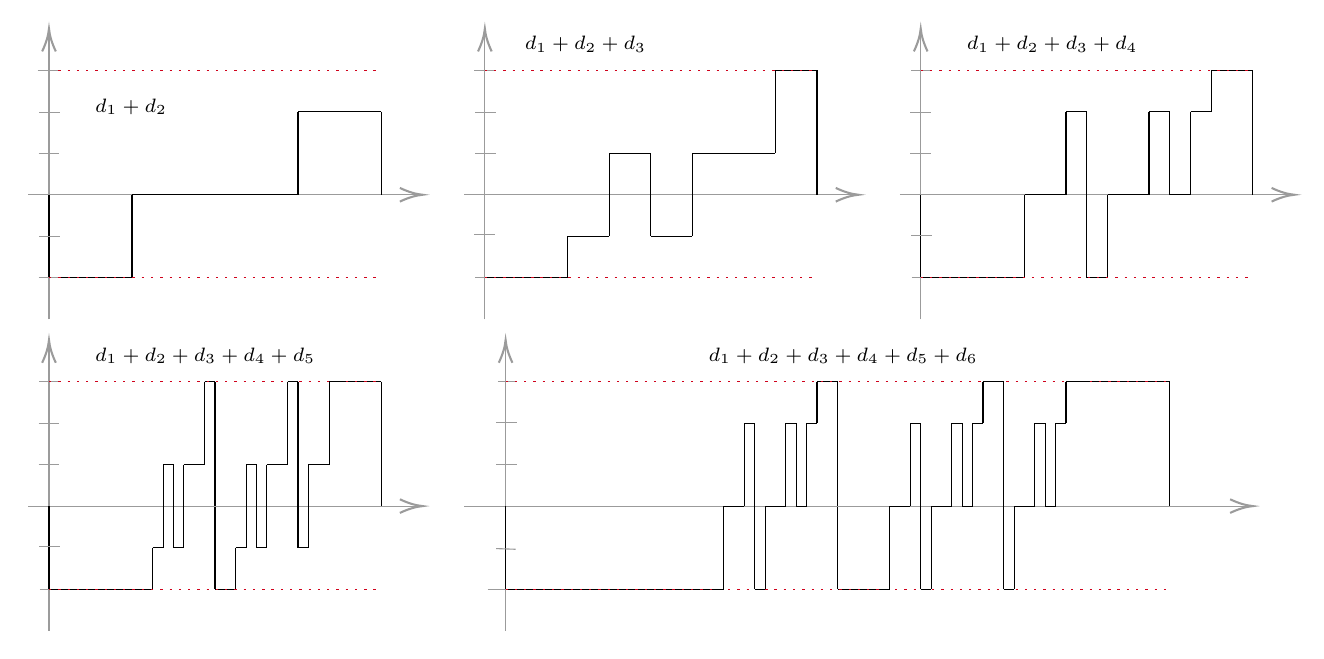
\begin{tikzpicture}[x=0.75pt,y=0.75pt,yscale=-1,xscale=1]
		%uncomment if require: \path (0,300); %set diagram left start at 0, and has height of 300
		
		%Straight Lines [id:da9280320279304022] 
		\draw [color={rgb, 255:red, 155; green, 155; blue, 155 }  ,draw opacity=1 ]   (230,150) -- (230,12) ;
		\draw [shift={(230,10)}, rotate = 90] [color={rgb, 255:red, 155; green, 155; blue, 155 }  ,draw opacity=1 ][line width=0.75]    (10.93,-3.29) .. controls (6.95,-1.4) and (3.31,-0.3) .. (0,0) .. controls (3.31,0.3) and (6.95,1.4) .. (10.93,3.29)   ;
		%Straight Lines [id:da9203900000578629] 
		\draw [color={rgb, 255:red, 155; green, 155; blue, 155 }  ,draw opacity=1 ]   (220,90) -- (408,90) ;
		\draw [shift={(410,90)}, rotate = 180] [color={rgb, 255:red, 155; green, 155; blue, 155 }  ,draw opacity=1 ][line width=0.75]    (10.93,-3.29) .. controls (6.95,-1.4) and (3.31,-0.3) .. (0,0) .. controls (3.31,0.3) and (6.95,1.4) .. (10.93,3.29)   ;
		%Straight Lines [id:da3920866977684767] 
		\draw    (290,70) -- (290,110) ;
		%Straight Lines [id:da3723218598502702] 
		\draw    (270,110) -- (290,110) ;
		%Straight Lines [id:da2571567869066207] 
		\draw    (290,70) -- (310,70) ;
		%Straight Lines [id:da6635517735775418] 
		\draw    (330,70) -- (330,110) ;
		%Straight Lines [id:da6227621396076539] 
		\draw    (310,110) -- (330,110) ;
		%Straight Lines [id:da031155489985427165] 
		\draw    (330,70) -- (350,70) ;
		%Straight Lines [id:da03018160126009639] 
		\draw    (370,30) -- (370,70) ;
		%Straight Lines [id:da09683216760785229] 
		\draw    (350,70) -- (370,70) ;
		%Straight Lines [id:da8197744855073605] 
		\draw    (370,30) -- (390,30) ;
		%Straight Lines [id:da9857640514641124] 
		\draw    (310,70) -- (310,110) ;
		%Straight Lines [id:da39421609482994024] 
		\draw    (390,30) -- (390,90) ;
		%Straight Lines [id:da07796556282404521] 
		\draw [color={rgb, 255:red, 155; green, 155; blue, 155 }  ,draw opacity=1 ]   (20,150) -- (20,12) ;
		\draw [shift={(20,10)}, rotate = 90] [color={rgb, 255:red, 155; green, 155; blue, 155 }  ,draw opacity=1 ][line width=0.75]    (10.93,-3.29) .. controls (6.95,-1.4) and (3.31,-0.3) .. (0,0) .. controls (3.31,0.3) and (6.95,1.4) .. (10.93,3.29)   ;
		%Straight Lines [id:da2563013092187161] 
		\draw [color={rgb, 255:red, 155; green, 155; blue, 155 }  ,draw opacity=1 ]   (10,90) -- (198,90) ;
		\draw [shift={(200,90)}, rotate = 180] [color={rgb, 255:red, 155; green, 155; blue, 155 }  ,draw opacity=1 ][line width=0.75]    (10.93,-3.29) .. controls (6.95,-1.4) and (3.31,-0.3) .. (0,0) .. controls (3.31,0.3) and (6.95,1.4) .. (10.93,3.29)   ;
		%Straight Lines [id:da08463779453359743] 
		\draw    (180,50) -- (180,90) ;
		%Straight Lines [id:da7750732388180797] 
		\draw    (20,90) -- (20,130) ;
		%Straight Lines [id:da08013615350186809] 
		\draw    (20,130) -- (60,130) ;
		%Straight Lines [id:da6066608771920363] 
		\draw    (60,90) -- (60,130) ;
		%Straight Lines [id:da060568511625674004] 
		\draw    (60,90) -- (100,90) ;
		%Straight Lines [id:da3874840699084394] 
		\draw    (100,90) -- (140,90) ;
		%Straight Lines [id:da3966628356006987] 
		\draw    (140,50) -- (140,90) ;
		%Straight Lines [id:da17902948494422977] 
		\draw    (140,50) -- (180,50) ;
		%Straight Lines [id:da3472182828631549] 
		\draw [color={rgb, 255:red, 155; green, 155; blue, 155 }  ,draw opacity=1 ]   (15.33,50.33) -- (25.33,50.33) ;
		%Straight Lines [id:da8432091041088066] 
		\draw [color={rgb, 255:red, 155; green, 155; blue, 155 }  ,draw opacity=1 ]   (225.33,70) -- (235.33,70) ;
		%Straight Lines [id:da06301911134053695] 
		\draw [color={rgb, 255:red, 155; green, 155; blue, 155 }  ,draw opacity=1 ]   (225.33,50.33) -- (235.33,50.33) ;
		%Straight Lines [id:da38196297279268365] 
		\draw [color={rgb, 255:red, 155; green, 155; blue, 155 }  ,draw opacity=1 ]   (225,30) -- (235,30) ;
		%Straight Lines [id:da4645800623199432] 
		\draw [color={rgb, 255:red, 155; green, 155; blue, 155 }  ,draw opacity=1 ]   (15,70) -- (25,70) ;
		%Straight Lines [id:da2910258013985927] 
		\draw [color={rgb, 255:red, 155; green, 155; blue, 155 }  ,draw opacity=1 ]   (15.33,110) -- (25.33,110) ;
		%Straight Lines [id:da6903782546627151] 
		\draw [color={rgb, 255:red, 155; green, 155; blue, 155 }  ,draw opacity=1 ]   (15,129.67) -- (25,129.67) ;
		%Straight Lines [id:da3210383214403192] 
		\draw [color={rgb, 255:red, 155; green, 155; blue, 155 }  ,draw opacity=1 ]   (225.33,129.67) -- (235.33,129.67) ;
		%Straight Lines [id:da38772385675410903] 
		\draw [color={rgb, 255:red, 155; green, 155; blue, 155 }  ,draw opacity=1 ]   (225,109.33) -- (235,109.33) ;
		%Straight Lines [id:da907188748089873] 
		\draw [color={rgb, 255:red, 208; green, 2; blue, 27 }  ,draw opacity=1 ] [dash pattern={on 0.84pt off 2.51pt}]  (20,130) -- (180,130) ;
		%Straight Lines [id:da2790674651129499] 
		\draw [color={rgb, 255:red, 208; green, 2; blue, 27 }  ,draw opacity=1 ] [dash pattern={on 0.84pt off 2.51pt}]  (20,30) -- (180,30) ;
		%Straight Lines [id:da08576356572217092] 
		\draw [color={rgb, 255:red, 155; green, 155; blue, 155 }  ,draw opacity=1 ]   (14.53,29.93) -- (24.53,29.93) ;
		%Straight Lines [id:da5820740995033273] 
		\draw    (230,130) -- (250,130) ;
		%Straight Lines [id:da32861230423368637] 
		\draw    (250,130) -- (270,130) ;
		%Straight Lines [id:da8269551553421162] 
		\draw    (270,110) -- (270,130) ;
		%Straight Lines [id:da6074102117832687] 
		\draw [color={rgb, 255:red, 208; green, 2; blue, 27 }  ,draw opacity=1 ] [dash pattern={on 0.84pt off 2.51pt}]  (230,130) -- (390,130) ;
		%Straight Lines [id:da03880443558253677] 
		\draw [color={rgb, 255:red, 208; green, 2; blue, 27 }  ,draw opacity=1 ] [dash pattern={on 0.84pt off 2.51pt}]  (230,30) -- (390,30) ;
		%Straight Lines [id:da7258779528736234] 
		\draw [color={rgb, 255:red, 155; green, 155; blue, 155 }  ,draw opacity=1 ]   (440,150) -- (440,12) ;
		\draw [shift={(440,10)}, rotate = 90] [color={rgb, 255:red, 155; green, 155; blue, 155 }  ,draw opacity=1 ][line width=0.75]    (10.93,-3.29) .. controls (6.95,-1.4) and (3.31,-0.3) .. (0,0) .. controls (3.31,0.3) and (6.95,1.4) .. (10.93,3.29)   ;
		%Straight Lines [id:da22546869153769022] 
		\draw [color={rgb, 255:red, 155; green, 155; blue, 155 }  ,draw opacity=1 ]   (430,90) -- (618,90) ;
		\draw [shift={(620,90)}, rotate = 180] [color={rgb, 255:red, 155; green, 155; blue, 155 }  ,draw opacity=1 ][line width=0.75]    (10.93,-3.29) .. controls (6.95,-1.4) and (3.31,-0.3) .. (0,0) .. controls (3.31,0.3) and (6.95,1.4) .. (10.93,3.29)   ;
		%Straight Lines [id:da6531287614930199] 
		\draw    (440,90) -- (440,130) ;
		%Straight Lines [id:da5081428422687104] 
		\draw    (600,30) -- (600,90) ;
		%Straight Lines [id:da11478333416409026] 
		\draw    (450,130) -- (460,130) ;
		%Straight Lines [id:da1291391061735716] 
		\draw    (460,130) -- (470,130) ;
		%Straight Lines [id:da03092960098427211] 
		\draw    (470,130) -- (480,130) ;
		%Straight Lines [id:da4348420247945328] 
		\draw    (490,90) -- (490,130) ;
		%Straight Lines [id:da604756945008629] 
		\draw    (480,130) -- (490,130) ;
		%Straight Lines [id:da697923574210926] 
		\draw    (490,90) -- (500,90) ;
		%Straight Lines [id:da27395623100833877] 
		\draw    (510,50) -- (510,90) ;
		%Straight Lines [id:da5103451563907193] 
		\draw    (500,90) -- (510,90) ;
		%Straight Lines [id:da6714783233517674] 
		\draw    (510,50) -- (520,50) ;
		%Straight Lines [id:da4750026840959556] 
		\draw    (530,90) -- (530,130) ;
		%Straight Lines [id:da5211152243871449] 
		\draw    (520,130) -- (530,130) ;
		%Straight Lines [id:da9621554662910814] 
		\draw    (530,90) -- (540,90) ;
		%Straight Lines [id:da3572367617670924] 
		\draw    (550,50) -- (550,90) ;
		%Straight Lines [id:da03686984083486422] 
		\draw    (540,90) -- (550,90) ;
		%Straight Lines [id:da61489257934252] 
		\draw    (550,50) -- (560,50) ;
		%Straight Lines [id:da7825569344208265] 
		\draw    (570,50) -- (570,90) ;
		%Straight Lines [id:da3201117537952136] 
		\draw    (560,90) -- (570,90) ;
		%Straight Lines [id:da11336523510308516] 
		\draw    (570,50) -- (580,50) ;
		%Straight Lines [id:da7488314780476206] 
		\draw    (580,30) -- (590,30) ;
		%Straight Lines [id:da5288652332117192] 
		\draw    (590,30) -- (600,30) ;
		%Straight Lines [id:da45873411151895604] 
		\draw    (520,50) -- (520,130) ;
		%Straight Lines [id:da6432126167020484] 
		\draw    (560,50) -- (560,90) ;
		%Straight Lines [id:da3195371031966625] 
		\draw [color={rgb, 255:red, 155; green, 155; blue, 155 }  ,draw opacity=1 ]   (435,70) -- (445,70) ;
		%Straight Lines [id:da2424254172571465] 
		\draw [color={rgb, 255:red, 155; green, 155; blue, 155 }  ,draw opacity=1 ]   (435,50.33) -- (445,50.33) ;
		%Straight Lines [id:da9533004294097529] 
		\draw [color={rgb, 255:red, 155; green, 155; blue, 155 }  ,draw opacity=1 ]   (435.33,30) -- (445.33,30) ;
		%Straight Lines [id:da12975233898780014] 
		\draw [color={rgb, 255:red, 155; green, 155; blue, 155 }  ,draw opacity=1 ]   (435.67,130) -- (445.67,130) ;
		%Straight Lines [id:da15521916311097583] 
		\draw [color={rgb, 255:red, 155; green, 155; blue, 155 }  ,draw opacity=1 ]   (435.33,109.67) -- (445.33,109.67) ;
		%Straight Lines [id:da32056524925840413] 
		\draw    (580,30) -- (580,50) ;
		%Straight Lines [id:da9874638292708502] 
		\draw    (440,130) -- (460,130) ;
		%Straight Lines [id:da49913919302757614] 
		\draw [color={rgb, 255:red, 208; green, 2; blue, 27 }  ,draw opacity=1 ] [dash pattern={on 0.84pt off 2.51pt}]  (440,130) -- (600,130) ;
		%Straight Lines [id:da22634272337086214] 
		\draw [color={rgb, 255:red, 208; green, 2; blue, 27 }  ,draw opacity=1 ] [dash pattern={on 0.84pt off 2.51pt}]  (440,30) -- (600,30) ;
		%Straight Lines [id:da0532577225715114] 
		\draw    (95,180) -- (95,220) ;
		%Straight Lines [id:da2354244707540114] 
		\draw    (90,220) -- (95,220) ;
		%Straight Lines [id:da03130665137204791] 
		\draw    (95,180) -- (100,180) ;
		%Straight Lines [id:da9382461032210963] 
		\draw    (100,180) -- (100,280) ;
		%Straight Lines [id:da4753049094377122] 
		\draw [color={rgb, 255:red, 155; green, 155; blue, 155 }  ,draw opacity=1 ]   (20,300) -- (20,162) ;
		\draw [shift={(20,160)}, rotate = 90] [color={rgb, 255:red, 155; green, 155; blue, 155 }  ,draw opacity=1 ][line width=0.75]    (10.93,-3.29) .. controls (6.95,-1.4) and (3.31,-0.3) .. (0,0) .. controls (3.31,0.3) and (6.95,1.4) .. (10.93,3.29)   ;
		%Straight Lines [id:da5502861510617474] 
		\draw [color={rgb, 255:red, 155; green, 155; blue, 155 }  ,draw opacity=1 ]   (10,240) -- (198,240) ;
		\draw [shift={(200,240)}, rotate = 180] [color={rgb, 255:red, 155; green, 155; blue, 155 }  ,draw opacity=1 ][line width=0.75]    (10.93,-3.29) .. controls (6.95,-1.4) and (3.31,-0.3) .. (0,0) .. controls (3.31,0.3) and (6.95,1.4) .. (10.93,3.29)   ;
		%Straight Lines [id:da849025746886827] 
		\draw    (20,240) -- (20,280) ;
		%Straight Lines [id:da8897103919924259] 
		\draw    (180,180) -- (180,240) ;
		%Straight Lines [id:da6460195332699319] 
		\draw    (30,280) -- (40,280) ;
		%Straight Lines [id:da8069141545352652] 
		\draw    (40,280) -- (50,280) ;
		%Straight Lines [id:da41302144634317894] 
		\draw    (50,280) -- (60,280) ;
		%Straight Lines [id:da07469519423695159] 
		\draw    (70,260) -- (70,280) ;
		%Straight Lines [id:da7022436602910578] 
		\draw    (60,280) -- (70,280) ;
		%Straight Lines [id:da5999455244008518] 
		\draw    (110,260) -- (110,280) ;
		%Straight Lines [id:da1844823970790046] 
		\draw    (100,280) -- (110,280) ;
		%Straight Lines [id:da34541246394360337] 
		\draw    (160,180) -- (170,180) ;
		%Straight Lines [id:da6042199909798041] 
		\draw    (170,180) -- (180,180) ;
		%Straight Lines [id:da7948140815078759] 
		\draw [color={rgb, 255:red, 155; green, 155; blue, 155 }  ,draw opacity=1 ]   (15,220) -- (25,220) ;
		%Straight Lines [id:da13143847289065214] 
		\draw [color={rgb, 255:red, 155; green, 155; blue, 155 }  ,draw opacity=1 ]   (15,200.33) -- (25,200.33) ;
		%Straight Lines [id:da13032469689208037] 
		\draw [color={rgb, 255:red, 155; green, 155; blue, 155 }  ,draw opacity=1 ]   (15.33,180) -- (25.33,180) ;
		%Straight Lines [id:da608663988838781] 
		\draw [color={rgb, 255:red, 155; green, 155; blue, 155 }  ,draw opacity=1 ]   (15.67,280) -- (25.67,280) ;
		%Straight Lines [id:da8137387534895955] 
		\draw [color={rgb, 255:red, 155; green, 155; blue, 155 }  ,draw opacity=1 ]   (15.33,259.67) -- (25.33,259.67) ;
		%Straight Lines [id:da40794824044760114] 
		\draw    (20,280) -- (40,280) ;
		%Straight Lines [id:da2333562618500511] 
		\draw [color={rgb, 255:red, 208; green, 2; blue, 27 }  ,draw opacity=1 ] [dash pattern={on 0.84pt off 2.51pt}]  (20,280) -- (180,280) ;
		%Straight Lines [id:da8695294322881548] 
		\draw [color={rgb, 255:red, 208; green, 2; blue, 27 }  ,draw opacity=1 ] [dash pattern={on 0.84pt off 2.51pt}]  (20,180) -- (180,180) ;
		%Straight Lines [id:da7562348985805987] 
		\draw    (75,220) -- (75,260) ;
		%Straight Lines [id:da979353565162449] 
		\draw    (70,260) -- (75,260) ;
		%Straight Lines [id:da09415914267580372] 
		\draw    (75,220) -- (80,220) ;
		%Straight Lines [id:da4290468168806587] 
		\draw    (80,220) -- (80,260) ;
		%Straight Lines [id:da23523805102529094] 
		\draw    (85,220) -- (85,260) ;
		%Straight Lines [id:da9351313356745559] 
		\draw    (80,260) -- (85,260) ;
		%Straight Lines [id:da03596149124660886] 
		\draw    (85,220) -- (90,220) ;
		%Straight Lines [id:da15691981238218133] 
		\draw    (80,220) -- (80,260) ;
		%Straight Lines [id:da9037356330312156] 
		\draw    (115,220) -- (115,260) ;
		%Straight Lines [id:da2970786187028067] 
		\draw    (110,260) -- (115,260) ;
		%Straight Lines [id:da28688030082350036] 
		\draw    (115,220) -- (120,220) ;
		%Straight Lines [id:da6209664812659323] 
		\draw    (120,220) -- (120,260) ;
		%Straight Lines [id:da06564189491141947] 
		\draw    (135,180) -- (135,220) ;
		%Straight Lines [id:da35296344505953736] 
		\draw    (130,220) -- (135,220) ;
		%Straight Lines [id:da31658316944522813] 
		\draw    (135,180) -- (140,180) ;
		%Straight Lines [id:da6489801022469033] 
		\draw    (140,180) -- (140,220) ;
		%Straight Lines [id:da8434983696029628] 
		\draw    (125,220) -- (125,260) ;
		%Straight Lines [id:da285490026334273] 
		\draw    (120,260) -- (125,260) ;
		%Straight Lines [id:da32482311775227] 
		\draw    (125,220) -- (130,220) ;
		%Straight Lines [id:da22366430850119134] 
		\draw    (145,220) -- (145,260) ;
		%Straight Lines [id:da789321831789974] 
		\draw    (140,260) -- (145,260) ;
		%Straight Lines [id:da6742251365368728] 
		\draw    (145,220) -- (150,220) ;
		%Straight Lines [id:da5641177929852843] 
		\draw    (140,220) -- (140,260) ;
		%Straight Lines [id:da5674595150190624] 
		\draw    (155,180) -- (155,220) ;
		%Straight Lines [id:da02354563658988562] 
		\draw    (150,220) -- (155,220) ;
		%Straight Lines [id:da13155516560029068] 
		\draw    (155,180) -- (160,180) ;
		%Straight Lines [id:da7313977748522908] 
		\draw    (390,180) -- (390,200) ;
		%Straight Lines [id:da6082370562951926] 
		\draw    (390,180) -- (400,180) ;
		%Straight Lines [id:da3682727636688272] 
		\draw    (400,180) -- (400,280) ;
		%Straight Lines [id:da9528440489075882] 
		\draw [color={rgb, 255:red, 155; green, 155; blue, 155 }  ,draw opacity=1 ]   (240,300) -- (240,162) ;
		\draw [shift={(240,160)}, rotate = 90] [color={rgb, 255:red, 155; green, 155; blue, 155 }  ,draw opacity=1 ][line width=0.75]    (10.93,-3.29) .. controls (6.95,-1.4) and (3.31,-0.3) .. (0,0) .. controls (3.31,0.3) and (6.95,1.4) .. (10.93,3.29)   ;
		%Straight Lines [id:da23012430559119035] 
		\draw [color={rgb, 255:red, 155; green, 155; blue, 155 }  ,draw opacity=1 ]   (220,240) -- (598,240) ;
		\draw [shift={(600,240)}, rotate = 180] [color={rgb, 255:red, 155; green, 155; blue, 155 }  ,draw opacity=1 ][line width=0.75]    (10.93,-3.29) .. controls (6.95,-1.4) and (3.31,-0.3) .. (0,0) .. controls (3.31,0.3) and (6.95,1.4) .. (10.93,3.29)   ;
		%Straight Lines [id:da6141045485590793] 
		\draw    (240,240) -- (240,280) ;
		%Straight Lines [id:da5487593615684154] 
		\draw    (560,180) -- (560,240) ;
		%Straight Lines [id:da09616351584678573] 
		\draw    (260,280) -- (280,280) ;
		%Straight Lines [id:da48977350141799914] 
		\draw    (280,280) -- (300,280) ;
		%Straight Lines [id:da555890669902602] 
		\draw    (300,280) -- (320,280) ;
		%Straight Lines [id:da7788422689540324] 
		\draw    (320,280) -- (340,280) ;
		%Straight Lines [id:da8939466893722274] 
		\draw    (400,280) -- (420,280) ;
		%Straight Lines [id:da06599337519330084] 
		\draw    (520,180) -- (540,180) ;
		%Straight Lines [id:da522706800106159] 
		\draw    (540,180) -- (560,180) ;
		%Straight Lines [id:da21609933786190538] 
		\draw [color={rgb, 255:red, 155; green, 155; blue, 155 }  ,draw opacity=1 ]   (235.6,220) -- (245.6,220) ;
		%Straight Lines [id:da5028375621113421] 
		\draw [color={rgb, 255:red, 155; green, 155; blue, 155 }  ,draw opacity=1 ]   (235.6,199.6) -- (245.6,199.6) ;
		%Straight Lines [id:da25002598386043284] 
		\draw [color={rgb, 255:red, 155; green, 155; blue, 155 }  ,draw opacity=1 ]   (236.27,180) -- (245.6,180) ;
		%Straight Lines [id:da12950228230177174] 
		\draw [color={rgb, 255:red, 155; green, 155; blue, 155 }  ,draw opacity=1 ]   (231.33,280) -- (251.33,280) ;
		%Straight Lines [id:da708331922279634] 
		\draw [color={rgb, 255:red, 155; green, 155; blue, 155 }  ,draw opacity=1 ]   (235.47,260.47) -- (244.8,260.8) ;
		%Straight Lines [id:da04263468021306416] 
		\draw    (240,280) -- (280,280) ;
		%Straight Lines [id:da613116876822936] 
		\draw [color={rgb, 255:red, 208; green, 2; blue, 27 }  ,draw opacity=1 ] [dash pattern={on 0.84pt off 2.51pt}]  (240,280) -- (560,280) ;
		%Straight Lines [id:da34384498656677764] 
		\draw [color={rgb, 255:red, 208; green, 2; blue, 27 }  ,draw opacity=1 ] [dash pattern={on 0.84pt off 2.51pt}]  (240,180) -- (560,180) ;
		%Straight Lines [id:da962148012825395] 
		\draw    (360,200) -- (360,280) ;
		%Straight Lines [id:da658549642089012] 
		\draw    (440,200) -- (440,280) ;
		%Straight Lines [id:da08010505247756616] 
		\draw    (470,180) -- (470,200) ;
		%Straight Lines [id:da521598619712252] 
		\draw    (470,180) -- (480,180) ;
		%Straight Lines [id:da41645063680298566] 
		\draw    (480,180) -- (480,220) ;
		%Straight Lines [id:da23255457847524674] 
		\draw    (480,220) -- (480,280) ;
		%Straight Lines [id:da8566156756949999] 
		\draw    (510,180) -- (510,200) ;
		%Straight Lines [id:da0626915531164014] 
		\draw    (510,180) -- (520,180) ;
		%Straight Lines [id:da21688421324656781] 
		\draw    (345,240) -- (345,280) ;
		%Straight Lines [id:da9742992418415592] 
		\draw    (340,280) -- (345,280) ;
		%Straight Lines [id:da5948324607025091] 
		\draw    (345,240) -- (350,240) ;
		
		%Straight Lines [id:da2925033566994024] 
		\draw    (355,200) -- (355,240) ;
		%Straight Lines [id:da8575869071995488] 
		\draw    (350,240) -- (355,240) ;
		%Straight Lines [id:da3806341812503031] 
		\draw    (355,200) -- (360,200) ;
		%Straight Lines [id:da034942460968923506] 
		\draw    (365,240) -- (365,280) ;
		%Straight Lines [id:da10799041865288772] 
		\draw    (360,280) -- (365,280) ;
		%Straight Lines [id:da06531870547777907] 
		\draw    (365,240) -- (370,240) ;
		%Straight Lines [id:da8661224733027266] 
		\draw    (375,200) -- (375,240) ;
		%Straight Lines [id:da7497434917130008] 
		\draw    (370,240) -- (375,240) ;
		%Straight Lines [id:da3948527608301926] 
		\draw    (375,200) -- (380,200) ;
		%Straight Lines [id:da5382922889546415] 
		\draw    (385,200) -- (385,240) ;
		%Straight Lines [id:da4838380364375632] 
		\draw    (380,240) -- (385,240) ;
		%Straight Lines [id:da9913320087648876] 
		\draw    (385,200) -- (390,200) ;
		%Straight Lines [id:da13989093595542745] 
		\draw    (380,200) -- (380,240) ;
		%Straight Lines [id:da010247707031058706] 
		\draw    (425,240) -- (425,280) ;
		%Straight Lines [id:da5200805642916344] 
		\draw    (420,280) -- (425,280) ;
		%Straight Lines [id:da4608809883945928] 
		\draw    (425,240) -- (430,240) ;
		%Straight Lines [id:da8557161664953221] 
		\draw    (435,200) -- (435,240) ;
		%Straight Lines [id:da12747844698073352] 
		\draw    (430,240) -- (435,240) ;
		%Straight Lines [id:da001772759376845734] 
		\draw    (435,200) -- (440,200) ;
		%Straight Lines [id:da9172244700477454] 
		\draw    (445,240) -- (445,280) ;
		%Straight Lines [id:da6051739295445682] 
		\draw    (440,280) -- (445,280) ;
		%Straight Lines [id:da6158999118637307] 
		\draw    (445,240) -- (450,240) ;
		%Straight Lines [id:da11172966681439078] 
		\draw    (455,200) -- (455,240) ;
		%Straight Lines [id:da8977351525874624] 
		\draw    (450,240) -- (455,240) ;
		%Straight Lines [id:da309832896154842] 
		\draw    (455,200) -- (460,200) ;
		%Straight Lines [id:da012046237302282492] 
		\draw    (465,200) -- (465,240) ;
		%Straight Lines [id:da045207297054142837] 
		\draw    (460,240) -- (465,240) ;
		%Straight Lines [id:da8894727133224287] 
		\draw    (465,200) -- (470,200) ;
		%Straight Lines [id:da7225802658810978] 
		\draw    (485,240) -- (485,280) ;
		%Straight Lines [id:da3077412713526617] 
		\draw    (480,280) -- (485,280) ;
		%Straight Lines [id:da8930864420582325] 
		\draw    (485,240) -- (490,240) ;
		%Straight Lines [id:da7294374006796644] 
		\draw    (495,200) -- (495,240) ;
		%Straight Lines [id:da01909301657172624] 
		\draw    (490,240) -- (495,240) ;
		%Straight Lines [id:da7351343643071311] 
		\draw    (495,200) -- (500,200) ;
		%Straight Lines [id:da5379680720480153] 
		\draw    (505,200) -- (505,240) ;
		%Straight Lines [id:da6304083775601768] 
		\draw    (500,240) -- (505,240) ;
		%Straight Lines [id:da47485474557146223] 
		\draw    (505,200) -- (510,200) ;
		%Straight Lines [id:da26579815231107573] 
		\draw    (500,200) -- (500,240) ;
		%Straight Lines [id:da4816390303089617] 
		\draw    (460,200) -- (460,240) ;
		
		% Text Node
		\draw (41,42.4) node [anchor=north west][inner sep=0.75pt]  [font=\scriptsize]  {$d_{1} +d_{2}$};
		% Text Node
		\draw (248,12.4) node [anchor=north west][inner sep=0.75pt]  [font=\scriptsize]  {$d_{1} +d_{2} +d_{3}$};
		% Text Node
		\draw (461,12.4) node [anchor=north west][inner sep=0.75pt]  [font=\scriptsize]  {$d_{1} +d_{2} +d_{3} +d_{4}$};
		% Text Node
		\draw (41,162.4) node [anchor=north west][inner sep=0.75pt]  [font=\scriptsize]  {$d_{1} +d_{2} +d_{3} +d_{4} +d_{5}$};
		% Text Node
		\draw (336.5,162.4) node [anchor=north west][inner sep=0.75pt]  [font=\scriptsize]  {$d_{1} +d_{2} +d_{3} +d_{4} +d_{5} +d_{6}$};
		
		
	\end{tikzpicture}
\end{figure}
\end{document}

